

In this section we first validate the proposed WAD approach by showing that it produces more accurate results compared to the existing approaches. Furthermore, we experimentally demonstrate with synthetic datasets that F1-score presents some limitations. We then perform comparative evaluations of the eight aforementioned models while studying the impact of data contamination $c$ and window size $p$.


\begin{table*}[!t]
    \caption{Comparison of WAD, PA, PA$\%K$ and RPA approaches with MCC and F1 score.}
    \label{tab:chap_3:wad_vs_rpa}
    \setlength\tabcolsep{2pt} 
    \small
    
    \begin{tabular*}{\hsize}{@{\extracolsep{\fill}} lccccccc}
    \toprule
    \bf Metric & \bf 0.05 & \bf 0.1 & \bf 0.15 & \bf 0.2 & \bf 0.25 & \bf 0.3 & \bf 0.5 \\
    \midrule
    \multicolumn{8}{c}{\bf MCC-Score} \\
    \midrule
    \bf PA & 95.31$_{(\pm0.02)}$ & 90.70$_{(\pm0.03)}$ & 86.13$_{(\pm0.01)}$ & 81.60$_{(\pm0.01)}$ & 77.11$_{(\pm0.02)}$ & 72.62$_{(\pm0.02)}$ & 54.11$_{(\pm0.03)}$ \\
    \bf RPA & 87.01$_{(\pm0.06)}$ & 76.34$_{(\pm0.07)}$ & 67.20$_{(\pm0.04)}$ & 59.17$_{(\pm0.08)}$ & 51.97$_{(\pm0.09)}$ & 43.35$_{(\pm0.09)}$ & 21.96$_{(\pm0.07)}$ \\
    \bf WAD$_{\alpha=0.8}$ & 97.93$_{(\pm0.02)}$ & 91.36$_{(\pm0.03)}$ & 80.80$_{(\pm0.07)}$ & 68.60$_{(\pm0.11)}$ & 56.48$_{(\pm0.20)}$ & 45.23$_{(\pm0.15)}$ & 0.13$_{(\pm0.13)}$ \\
    \bf PA$\%K_{K=80}$ & 93.38$_{(\pm0.03)}$ & 81.94$_{(\pm0.02)}$ & 65.74$_{(\pm0.07)}$ & 47.36$_{(\pm0.10)}$ & 28.66$_{(\pm0.16)}$ & 10.50$_{(\pm0.11)}$ & -46.37$_{(\pm0.07)}$ \\
    \bf WAD$_{\alpha=0.9}$ & 90.62$_{(\pm0.07)}$ & 74.56$_{(\pm0.08)}$ & 59.19$_{(\pm0.08)}$ & 46.18$_{(\pm0.05)}$ & 35.51$_{(\pm0.06)}$ & 26.78$_{(\pm0.09)}$ & 0.15$_{(\pm0.06)}$ \\
    \bf PA$\%K_{K=90}$ & 85.61$_{(\pm0.05)}$ & 63.81$_{(\pm0.07)}$ & 42.11$_{(\pm0.08)}$ & 22.09$_{(\pm0.03)}$ & 3.96$_{(\pm0.06)}$ & -12.09$_{(\pm0.09)}$ & -51.71$_{(\pm0.06)}$ \\
    \bf WAD$_{\alpha=1}$ & 64.30$_{(\pm0.08)}$ & 44.79$_{(\pm0.11)}$ & 32.07$_{(\pm0.09)}$ & 23.03$_{(\pm0.05)}$ & 16.40$_{(\pm0.09)}$ & 11.39$_{(\pm0.08)}$ & 0.04$_{(\pm0.19)}$ \\
    \bf PA$\%K_{K=100}$ & 58.97$_{(\pm0.05)}$ & 33.37$_{(\pm0.09)}$ & 13.37$_{(\pm0.09)}$ & -03.02$_{(\pm0.06)}$ & -16.08$_{(\pm0.10)}$ & -26.28$_{(\pm0.11)}$ & -52.06$_{(\pm0.09)}$ \\
    \midrule
    \multicolumn{8}{c}{\bf F1-Score} \\
    \midrule
    \bf PA & 98.06$_{(\pm0.01)}$ & 96.19$_{(\pm0.01)}$ & 94.36$_{(\pm0.01)}$ & 92.60$_{(\pm0.01)}$ & 90.89$_{(\pm0.02)}$ & 89.23$_{(\pm0.02)}$ & 82.99$_{(\pm0.02)}$ \\
    \bf RPA & 89.29$_{(\pm0.06)}$ & 80.31$_{(\pm0.07)}$ & 72.63$_{(\pm0.06)}$ & 66.02$_{(\pm0.09)}$ & 60.28$_{(\pm0.10)}$ & 55.23$_{(\pm0.10)}$ & 39.88$_{(\pm0.08)}$ \\
    \bf WAD$_{\alpha=0.8}$ & 99.04$_{(\pm0.01)}$ & 95.72$_{(\pm0.02)}$ & 89.34$_{(\pm0.05)}$ & 79.95$_{(\pm0.09)}$ & 68.05$_{(\pm0.19)}$ & 54.56$_{(\pm0.17)}$ & 10.00$_{(\pm0.07)}$ \\
    \bf PA$\%K_{K=80}$ & 97.31$_{(\pm0.01)}$ & 92.44$_{(\pm0.01)}$ & 84.81$_{(\pm0.04)}$ & 74.63$_{(\pm0.06)}$ & 62.60$_{(\pm0.13)}$ & 49.79$_{(\pm0.11)}$ & 12.15$_{(\pm0.07)}$ \\
    \bf WAD$_{\alpha=0.9}$ & 95.20$_{(\pm0.04)}$ & 84.42$_{(\pm0.06)}$ & 70.10$_{(\pm0.08)}$ & 54.23$_{(\pm0.06)}$ & 38.91$_{(\pm0.08)}$ & 25.75$_{(\pm0.12)}$ & 2.11$_{(\pm0.04)}$ \\
    \bf PA$\%K_{K=90}$ & 93.72$_{(\pm0.03)}$ & 82.14$_{(\pm0.05)}$ & 67.79$_{(\pm0.06)}$ & 52.78$_{(\pm0.03)}$ & 39.04$_{(\pm0.07)}$ & 27.74$_{(\pm0.08)}$ & 7.48$_{(\pm0.05)}$ \\
    \bf WAD$_{\alpha=1}$ & 74.89$_{(\pm0.08)}$ & 51.60$_{(\pm0.16)}$ & 32.85$_{(\pm0.13)}$ & 19.40$_{(\pm0.06)}$ & 10.69$_{(\pm0.10)}$ & 5.49$_{(\pm0.06)}$ & 0.19$_{(\pm0.02)}$ \\
    \bf PA$\%K_{K=100}$ & 75.93$_{(\pm0.06)}$ & 54.66$_{(\pm0.13)}$ & 38.24$_{(\pm0.12)}$ & 26.74$_{(\pm0.06)}$ & 19.25$_{(\pm0.08)}$ & 14.53$_{(\pm0.09)}$ & 7.18$_{(\pm0.07)}$ \\
    \addlinespace
    \bottomrule
    \end{tabular*}
\end{table*}




\subsection{Comparison of WAD with existing approaches}\label{wad_metrics}

In this section, we show that the WAD approach can yield more accurate performance results compared to existing approaches. We then define a synthetic anomaly detection model that produce a rate $\beta$ of detection errors on the test set. Specifically, this AD model has an incorrect prediction for $\beta*100$ observations over a set of 100 observations. We refer to this model as \textit{$(1-\beta)$-perfect detector}, which is perfect when $\beta=0$ and is always wrong when $\beta=1$. We select different values for $\beta \in \{0.05,0.1,0.15,0.2,0.25,0.3,0.5\}$ and compute F1-score and MCC score accordingly. Table \ref{tab:chap_3:wad_vs_rpa} depicts the F1 and MCC score of the $(1-\beta)$-perfect detector for the WAD approach.

We notice that both MCC and F1-scores decrease for each window approach as the error rate of the synthetic model increases. On the one hand, when $\beta$ varies from 0.05 to 0.25, PA still gives high scores to the model (from a F1-score of 98\% to 90\%), while RPA results in low scores (from a F1-score of 89\% to 60\%). On the other hand, WAD$_{\alpha=0.8}$ and PA$\%K_{K=80}$ strike a balance to provide a more accurate reflection of model quality.
%, realize a trade-off to better reflect the model quality. 
For instance, MCC score decreases from 98\% to 56\% for WAD and from 93\% to 28\% for PA$\%K$. Both approaches increase their penalization as $\beta$ increases. However, when $\beta$ reaches 0.5, which corresponds to random predictions, WAD approach reports an MCC score of 0\%, while PA$\%K$ continues to penalize the model and produces negative MCC scores (worse than a random model). The reason behind this behavior of PA$\%K$ is related to its way of adjusting differently for anomalous and normal segments prediction compared to WAD approach, which handles both segment types similarly.

As for the PA$\%K$ approach, the score reported with WAD also depends on a tolerance parameter, here $\alpha$. Increasing $\alpha$ from 0.8 to 1, results in low scores, even lower than those reported with RPA on a near-perfect model. For instance, a model with a low error rate ($\beta=0.05$) and WAD with tolerance $\alpha=1$, achieves an F1-score of 74\%, while the PA and RPA approaches report a F1-score of 98\% and 89\%, respectively. We obtain such scores because with a tolerance $\alpha=1$, only models that can detect all anomalies in the window get high scores.

\takeaway{Unlike PA, PA$\%K$ and RPA, the WAD approach offers a more accurate evaluation of model performance by equally adjusting the prediction for anomalous and normal segments and the score obtained by a model is proportional to its ability to accurately detect a sequence of anomalous observations long enough to be severe.} %and then worth reported by the monitoring system and proportionally to the desired tolerance.}

\begin{table}[!t]
    \caption{Comparison between F1-score and MCC computed on synthetic AD models.}
    \label{tab:chap_3:mcc_vs_f1}
    \setlength\tabcolsep{0pt} 
    
    \begin{tabular*}{\hsize}{@{\extracolsep{\fill}} llcccc}
    \toprule
        \bf Model & \bf Window approach & \bf Precision & \bf Recall & \bf F1-score & \bf MCC \\
    \midrule
        \multirow{6}{*}{\rotatebox[origin=c]{90}{\bf Zero-rule}} & \bf PW & 58.38   & 100 & 73.72   & 0.0 \\
        & \bf PA & 58.38   & 100 & 73.72   & 0.0 \\
        & \bf RPA & 19.06   & 100 & 32.02   & 0.0 \\
        & \bf WAD$_{\alpha=0.8}$ & 54.34 & 100 & 70.41 & 0.0 \\
        & \bf PA$\%K_{K=80}$ & 58.38 & 100 & 73.72 & 0.0 \\
       % & \bf WAD$_{\alpha=0.9}$ & 53.54 & 100 & 69.74 & 0.0 \\
        & \bf WAD$_{\alpha=1}$ & 52.57 & 100 & 68.92 & 0.0 \\
        & \bf PA$\%K_{K=100}$ & 58.38 & 100 & 73.72 & 0.0 \\
    \midrule
        \multirow{6}{*}{\rotatebox[origin=c]{90}{\bf Random}} & \bf PW & 58.37 & 49.97 & 53.89   & 0.0 \\
        & \bf PA & 73.97 & 96.20 & 82.99 & 54.10  \\
        & \bf RPA & 28.61 & 77.77 & 39.88 & 21.95 \\
        & \bf WAD$_{\alpha=0.8}$ & 54.32 & 5.47 & 9.94 & -0.01 \\
        & \bf PA$\%K_{K=80}$ & 19.70 & 8.74 & 12.11 & -46.40 \\
        %& \bf WAD$_{\alpha=0.9}$ & 53.62   & 1.08   & 2.11   & 0.02   \\
        & \bf WAD$_{\alpha=1}$ & 52.19 & 0.10 & 0.20 & -0.03   \\
        & \bf PA$\%K_{K=80}$ & 12.40 & 5.05 & 7.18 & -52.06 \\
    
    
    \addlinespace
    \bottomrule
    \end{tabular*}
    \end{table}



\subsection{Comparison between F1-score and MCC}

We compare in this section the F1-score and MCC metrics on synthetic anomaly detection models. We first consider a \textit{zero-rule} model that always outputs $\tilde{y_t} = 1 \text{ } \forall \text{ }{\tilde{x_t}}$  (i.e., this model always classifies any input $\tilde{x_t}$  as an anomaly). This model, if deployed,  triggers false alarms and may introduce high anomaly mitigation costs. We report the F1-score and the MCC of the \textit{zero-rule} model on our datasets with each window approach strategy in Table \ref{tab:chap_3:mcc_vs_f1}.


The results of Table \ref{tab:chap_3:mcc_vs_f1} show that F1-score reports higher scores ($\sim 70\%$) for each window approach (except for RPA), while the MCC reports a score of $0\%$ (i.e., worse than a tossing coin classifier) regardless of the approach. High F1-scores are mainly due to perfect recall scores, i.e., the model detects all the anomalies in the datasets.  But these F1-scores are misleading as the model identifies many normal instances as anomalous and then outputs a high number of false positives but no true negatives, which are not taken into account the F1-score. Consequently, when evaluating models having a low rate of true negatives, the F1-score metric should be carefully used.

Furthermore, we make the same observations in Table \ref{tab:chap_3:mcc_vs_f1} with a random guessing model. Indeed, we notice that F1-score is higher than MCC score, particularly for each approach. For instance, F1-score reported with PA (resp. WAD$_{\alpha=0.8}$) is 83\% (resp. 9.9\%), while the MCC score is 54\% (resp. 0\%). Since PA is known to overestimate the model performance, we also compute the F1-score and the MCC with the PW approach which are 53\% and 0\% respectively. The high F1-score obtained with this model regardless of the approach used asserts the observations made with zero-rule model.

\takeaway{If considering all conditions (TP, TN, FP, FN)  of the models is required, the MCC score should be preferred over the F1-score. The results of this experiment confirm the conclusions drawn by Chicco et al. \cite{Chicco2020TheAO}. In general, we recommend to use the MCC score and F1-score metrics together to avoid unreliable conclusions.} 




\begin{figure*}[!t]
    \centering
    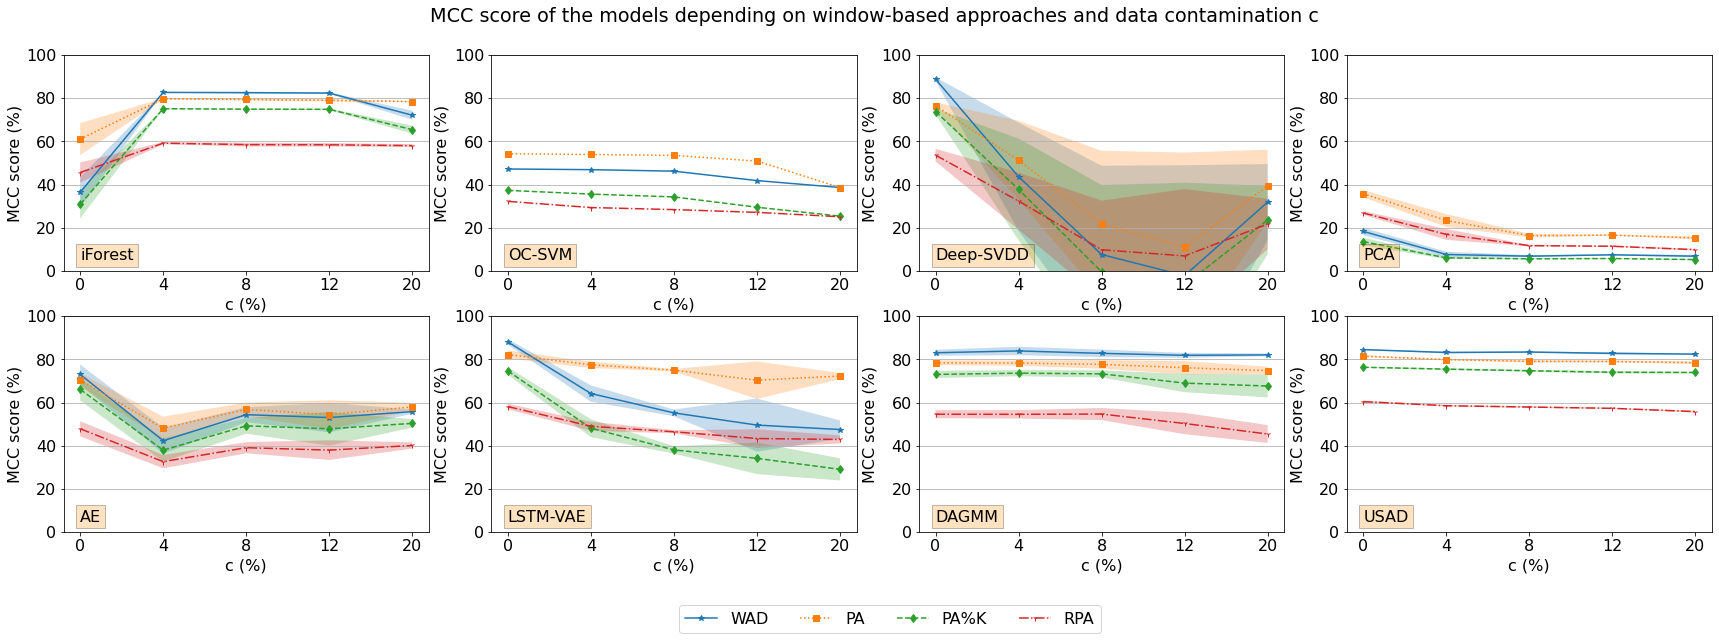
\includegraphics[width=\textwidth]{imgs/chapter_3/mcc_data_cont_approach.png}
    \caption{MCC score of unsupervised ML models with STD dataset according to the evaluation window-based approaches and the data contamination ratio $c$.}
    \label{fig:chap_3:mcc_app_cont_impact}
\end{figure*}

\subsection{Data contamination impact on unsupervised models}\label{data_conta}

\begin{table*}[ht!]

    \setlength\tabcolsep{1pt} 
    \footnotesize
    \begin{tabular*}{\textwidth}{@{\extracolsep{\fill}} lcc  cc c cc c cc}
    %\toprule
        & & & \multicolumn{2}{c}{\bf STD} &  & \multicolumn{2}{c}{\bf GFN} &  & \multicolumn{2}{c}{\bf XC}\\
    \cmidrule{4-5} \cmidrule{7-8} \cmidrule{10-11}
         & \bf Models & \bf $c$ (\%) & \bf F1 & \bf MCC &  & \bf F1 & \bf MCC &  & \bf F1 & \bf MCC \\
    
    \midrule
        \multirow{6}{*}{\rotatebox[origin=c]{90}{\bf Isolation-based}} & \multirow{5}{*}{\bf iForest} & \bf 0 & 48.68$_{\bf(\pm9.33)}$ & 36.45$_{(\pm6.97)}$ & & 25.65$_{(\pm2.19)}$ & 19.20$_{(\pm1.74)}$ & & \bf 54.36$_{\bf(\pm3.26)}$ & \bf 48.60$_{\bf(\pm2.82)}$ \\
                                & & \bf 4 & \bf 90.99$_{\bf(\pm0.12)}$ & \bf 82.70$_{\bf(\pm0.19)}$ & & 49.89$_{(\pm0.89)}$ & 37.26$_{(\pm0.72)}$ & & 49.69$_{(\pm3.40)}$ &  44.34$_{(\pm2.96)}$ \\
                                & & \bf 8 & 90.93$_{\bf(\pm0.15)}$ & 82.59$_{(\pm0.40)}$& & \bf 50.15$_{\bf(\pm0.85)}$ & \bf 37.49$_{\bf(\pm0.36)}$ & & 48.66$_{(\pm3.20)}$ & 44.34$_{(\pm2.43)}$ \\
                                & & \bf 12 & 90.82$_{(\pm0.19)}$ & 82.39$_{(\pm0.36)}$ & & 48.58$_{(\pm0.25)}$ & 36.42$_{(\pm0.38)}$ & & 46.01$_{(\pm2.26)}$ & 42.37$_{(\pm2.28)}$  \\
                                & & \bf 20 & 83.77$_{(\pm1.48)}$ & 72.13$_{(\pm2.11)}$ & & 48.00$_{(\pm0.46)}$ & 36.16$_{(\pm0.36)}$ & & 43.39$_{(\pm1.46)}$ & 40.98$_{(\pm1.34)}$  \\
                                & & & & & & & & & & \\
    \addlinespace    
    \midrule
        \multirow{10}{*}{\rotatebox[origin=c]{90}{\bf One-class classification}} & \multirow{5}{*}{\bf OC-SVM} & \bf 0 & \bf 77.67 & \bf 47.24 & & \bf 69.88 & \bf 29.41 & & \bf 66.27 & \bf 51.79 \\
                                & & \bf 4 & 77.35 & 46.93 & & 70.37 & 30.36 & & 65.15 & 48.51 \\
                                & & \bf 8 & 76.79 & 46.23 & & 68.68 & 28.24 & & 64.18 & 46.60 \\
                                & & \bf 12 & 74.20 & 41.87 & & 67.02 & 26.19 & & 63.32 & 44.98 \\
                                & & \bf 20 & 71.77 & 38.66 & & 63.47 & 21.78 & & 62.03 & 42.65 \\
    \addlinespace    
    \cmidrule{2-11}
        & \multirow{5}{*}{\bf Deep-SVDD} & \bf 0 & \bf 90.91$_{\bf(\pm0.59)}$ & \bf 88.85$_{\bf(\pm0.83)}$ & & 66.07$_{(\pm7.34)}$ & 8.69$_{(\pm20.27)}$ & & 49.61$_{(\pm14.19)}$ & 31.72$_{(\pm19.7)}$  \\
                                & & \bf 4 & 74.05$_{(\pm10.99)}$ & 43.64$_{(\pm25.11)}$ & & 67.49$_{(\pm4.78)}$ & 12.07$_{(\pm13.27)}$ & & 46.57$_{(\pm17.96)}$ & 23.9$_{(\pm26.11)}$ \\
                                & & \bf 8 & 56.48$_{(\pm19.1)}$& 7.63$_{(\pm41.11)}$ & & 65.03$_{(\pm6.16)}$ & 5.82$_{(\pm16.13)}$ & & \bf 62.87$_{\bf(\pm13.46)}$ & \bf 46.74$_{\bf(\pm19.20)}$ \\
                                & & \bf 12 & 53.08$_{(\pm23.06)}$ & -2.13$_{(\pm51.12)}$ & & 67.44$_{(\pm6.68)}$ & 11.69$_{(\pm19.17)}$ & & 37.07$_{(\pm7.59)}$ & 13.64$_{(\pm9.18)}$ \\
                                & & \bf 20 & 68.82$_{(\pm7.65)}$& 31.9$_{(\pm17.65)}$ & & \bf 68.3$_{\bf(\pm7.69)}$ & \bf 13.34$_{\bf(\pm21.11)}$ & & 34.8$_{(\pm10.89)}$ & 7.70$_{(\pm15.14)}$ \\
    \addlinespace    
    \midrule
        \multirow{25}{*}{\rotatebox[origin=c]{90}{\bf  Reconstruction-based}} &
        \multirow{5}{*}{\bf PCA} & \bf 0 & \bf 61.79$_{\bf(\pm0.90)}$& \bf 18.33$_{\bf(\pm1.73)}$ & & \bf 63.59$_{\bf(\pm0.52)}$ & \bf 1.89$_{\bf(\pm0.81)}$ & & \bf 36.38$_{(\pm0.29)}$ & \bf 10.96$_{\bf(\pm0.25)}$  \\
                                & & \bf 4 & 58.26$_{(\pm0.21)}$ & 7.64$_{(\pm1.29)}$ & & 63.13$_{(\pm0.70)}$ & -2.40$_{(\pm0.97)}$ & & 33.32$_{(\pm0.24)}$ & 6.63$_{(\pm0.35)}$ \\
                                & & \bf 8 & 58.80$_{(\pm0.24)}$ & 6.87$_{(\pm0.49)}$ & & 63.56$_{(\pm0.26)}$ & -2.19$_{(\pm0.52)}$ & & 33.85$_{(\pm0.66)}$ & 7.58$_{(\pm0.79)}$  \\
                                & & \bf 12 & 58.92$_{(\pm0.13)}$ & 7.50$_{(\pm0.25)}$ & & 63.62$_{(\pm0.28)}$ & -1.96$_{(\pm0.58)}$ & & 34.53$_{(\pm0.43)}$ & 8.45$_{(\pm0.41)}$  \\
                                & & \bf 20 & 58.66$_{(\pm0.14)}$ & 6.87$_{(\pm0.58)}$ & & 63.13$_{(\pm0.16)}$ & -3.25$_{(\pm0.24)}$ & & 35.43$_{(\pm0.39)}$ & 9.42$_{(\pm0.58)}$  \\
    \addlinespace    
    \cmidrule{2-11}
        & \multirow{5}{*}{\bf AE} & \bf 0 & \bf 86.73$_{\bf(\pm2.04)}$ & \bf 73.05$_{\bf(\pm4.61)}$ & & \bf 79.44$_{\bf(\pm4.08)}$ & \bf 47.17$_{\bf(\pm10.72)}$ & & \bf 76.84$_{\bf(\pm6.48)}$ & \bf 68.12$_{\bf(\pm8.43)}$ \\
                                & & \bf 4 & 74.09$_{(\pm2.56)}$ & 42.38$_{(\pm6.03)}$ & & 65.38$_{(\pm1.65)}$ & 10.98$_{(\pm4.32)}$ & & 49.23$_{(\pm10.70)}$ & 30.97$_{(\pm15.82)}$ \\
                                & & \bf 8 & 79.01$_{(\pm1.85)}$ & 54.44$_{(\pm3.47)}$ & & 65.11$_{(\pm1.29)}$ & 10.02$_{(\pm2.25)}$ & & 40.77$_{(\pm2.66)}$ & 18.98$_{(\pm2.63)}$ \\
                                & & \bf 12 & 78.29$_{(\pm3.32)}$ & 53.1$_{(\pm6.84)}$ & & 64.34$_{(\pm2.42)}$ & 8.36$_{(\pm4.97)}$ & & 45.74$_{(\pm8.53)}$ & 25.25$_{(\pm11.12)}$  \\
                                & & \bf 20 & 79.67$_{(\pm0.86)}$ & 55.85$_{(\pm0.99)}$ & & 64.48$_{(\pm2.11)}$ & 6.59$_{(\pm6.83)}$ & & 42.98$_{(\pm2.75)}$ & 21.15$_{(\pm3.36)}$  \\
    \addlinespace    
    \cmidrule{2-11}
        & \multirow{5}{*}{\bf LSTM-VAE} & \bf 0 & \bf 94.44$_{\bf(\pm0.57)}$ & \bf 88.13$_{\bf(\pm1.30)}$ & & \bf 79.30$_{\bf(\pm0.63)}$ & \bf 50.68$_{\bf(\pm1.65)}$ & & \bf 64.15$_{\bf(\pm12.44)}$ &\bf 54.95$_{\bf(\pm11.11)}$  \\
                                & & \bf 4 & 81.9$_{(\pm2.02)}$ & 64.23$_{(\pm3.78)}$ & & 76.87$_{(\pm0.45)}$ & 43.28$_{(\pm0.84)}$ & & 63.50$_{(\pm2.31)}$ & 51.90$_{(\pm3.41)}$ \\
                                & & \bf 8 & 76.51$_{(\pm0.93)}$ & 55.26$_{(\pm1.56)}$ & & 74.94$_{(\pm1.23)}$ & 38.09$_{(\pm3.25)}$ & & 59.05$_{(\pm4.17)}$ & 45.65$_{(\pm4.99)}$ \\
                                & & \bf 12 & 74.14$_{(\pm5.12)}$ & 49.61$_{(\pm12.3)}$ & & 73.00$_{(\pm1.58)}$ & 34.56$_{(\pm4.25)}$ & & 57.75$_{(\pm0.53)}$ & 44.44$_{(\pm0.65)}$  \\
                                & & \bf 20 & 71.91$_{(\pm2.62)}$ & 47.55$_{(\pm4.23)}$ & & 70.28$_{(\pm0.86)}$ & 31.24$_{(\pm1.88)}$  & & 53.29$_{(\pm1.82)}$ & 39.16$_{(\pm2.85)}$  \\
    \addlinespace    
    \cmidrule{2-11}
        & \multirow{5}{*}{\bf DAGMM} & \bf 0 & 91.23$_{(\pm0.71)}$ & 83.11$_{(\pm1.37)}$ & & \bf 74.31$_{\bf(\pm1.86)}$ & \bf 32.08$_{\bf(\pm3.64)}$ & & \bf 68.10$_{\bf(\pm2.82)}$ & \bf 55.76$_{\bf(\pm3.82)}$  \\
                                & & \bf 4 & \bf 91.84$_{\bf(\pm0.77)}$ & \bf 83.95$_{\bf(\pm1.96)}$ & & 76.72$_{(\pm1.81)}$ & 38.08$_{(\pm3.87)}$ & & 66.16$_{(\pm1.34)}$ & 53.18$_{(\pm2.13)}$ \\
                                & & \bf 8 & 91.50$_{(\pm0.79)}$ & 82.83$_{(\pm1.74)}$ & & 75.09$_{(\pm3.04)}$ & 34.47$_{(\pm7.15)}$ & & 63.02$_{(\pm2.98)}$ & 49.17$_{(\pm3.80)}$ \\
                                & & \bf 12 & 91.33$_{(\pm0.48)}$ & 81.92$_{(\pm1.12)}$ & & 73.86$_{(\pm2.9)}$ & 31.32$_{(\pm7.31)}$ & & 63.04$_{(\pm2.48)}$ & 49.14$_{(\pm3.20)}$  \\
                                & & \bf 20 & 91.43$_{(\pm0.3)}$ & 82.12$_{(\pm0.65)}$ & & 71.66$_{(\pm3.16)}$ & 24.80$_{(\pm6.55)}$ & & 60.10$_{(\pm3.14)}$ & 45.54$_{(\pm4.05)}$  \\
    \addlinespace    
    \cmidrule{2-11}
        & \multirow{5}{*}{\bf USAD} & \bf 0 & \bf 92.79$_{\bf(\pm0.11)}$ & \bf 84.57$_{\bf(\pm0.20)}$& & \bf 76.73$_{\bf(\pm0.41)}$ & \bf 38.77$_{\bf(\pm1.03)}$ & & \bf 73.27$_{\bf(\pm1.52)}$ & \bf 62.30$_{\bf(\pm1.87)}$ \\
                                & & \bf 4 & 92.09$_{(\pm0.20)}$& 83.23$_{(\pm0.41)}$ & & 76.64$_{(\pm0.66)}$ & 38.04$_{(\pm1.56)}$  & & 65.74$_{(\pm1.56)}$ & 52.60$_{(\pm2.03)}$  \\
                                & & \bf 8 & 91.78$_{(\pm0.14)}$ & 83.44$_{(\pm0.28)}$ & & 75.25$_{(\pm0.77)}$ & 34.31$_{(\pm2.80)}$ & & 65.16$_{(\pm3.45)}$ & 51.77$_{(\pm4.31)}$  \\
                                & & \bf 12 & 91.63$_{(\pm0.08)}$ & 82.82$_{(\pm0.55)}$ & & 75.06$_{(\pm0.38)}$ & 33.69$_{(\pm1.03)}$ & & 61.24$_{(\pm4.49)}$ & 47.97$_{(\pm4.65)}$  \\
                                & & \bf 20 & 91.36$_{(\pm0.17)}$ & 82.48$_{(\pm0.13)}$ & & 74.64$_{(\pm1.30)}$ & 32.23$_{(\pm2.99)}$ & & 61.06$_{(\pm5.74)}$ & 46.38$_{(\pm7.02)}$  \\
    \addlinespace    
    \bottomrule
    \end{tabular*}
    \caption{Overall performance (mean and standard deviations over 5 runs) according to the training set's data contamination ratio $c$ and using the WAD approaches on the 3 datasets. Bold values indicate the best score for each model.}
    \label{tab:chap_3:performance_contamination}
    \end{table*}




This section presents the evaluation results for the eight unsupervised ML models. We first present the impact of data contamination on the performance of these models while using window-based approaches (WAD, PA, PA$\%K$ and RPA). Fig. \ref{fig:chap_3:mcc_app_cont_impact} depicts the variation of their MCC scores using data contamination ratio $c \in \{0\%,4\%,8\%,12\%,20\%\}$ on the STD dataset. We choose these values for data contamination as there are only few anomalies encountered in production networks, and these values are those encountered in previous works \cite{Johari2022AnomalyDA,Nkashama2022RobustnessEO}. We go up to 20\% to stress the models.


As depicted in Fig \ref{fig:chap_3:mcc_app_cont_impact}, data contamination impacts the ML models differently depending on the model family. Isolation-based models appear to benefit from data contamination. iForest shows low MCC score when there is no data contamination. Its performance largely increases with data contamination $c=4\%$ and slightly decreases as data contamination ratio increases. This is the expected behavior of iForest which assumes that anomalies are present in the training set but in few quantity and starkly differ from normal instances. The presence of anomalies helps iForest during training but with the increasing anomalies in training set, its performance drops when $c$ reaches 20\%. Therefore, the iForest can not efficiently isolate anomalies when there are a lot of anomalies in the training set.

One-class classification models, OC-SVM and Deep-SVDD, have their best performance with no data contamination (MCC$_{WAD}$ of 47.24\% and 88.65\%, respectively for instance). However, their performance decreases when anomalies are included in the training set. MCC score of OC-SVM slightly decreases and remains at a similar level. Surprisingly, Deep-SVDD performance (which has the best MCC score among all the models without data contamination), drops significantly and becomes even worse than a random classifier when $c=12\%$ (i.e., MCC$_{WAD} =-2\%$) and presents high standard deviations errors (i.e., 51\%). 
Deep-SVDD, although being a neural implementation of OC-SVM with the same objective function, presents high variability in results from one run to another. Moreover, it is difficult to contrast these results on Deep-SVDD with previous works as there is, to the best of our knowledge, either no work on data contamination impact with time-series data using Deep-SVDD or the existing works focus on image datasets. % Ref à ajouter


Reconstruction-based models present two different behavior when facing data contamination. On one hand, we note that PCA, AE and LSTM-VAE are less robust to the presence of anomalies in the training set. PCA, which is the less efficient model for anomaly detection, achieves a MCC$_{WAD}$ score of 18\% when $c=0\%$ which drops to 7\% when $c=4\%$. From this contamination level, increasing the rate of anomalies seems to have no significant impact on the PCA model, as its performance remains at the same level. AE and LSTM-VAE report a MCC$_{WAD}$ score of 73\% and 88\%, respectively which decreases to 55\% and 47\%, respectively, when data contamination ratio reaches $c=20\%$. AE and LSTM-VAE are the most impacted models to data contamination since a contamination ratio of $c=4\%$ is enough to deteriorate their performance by up to 30\%. On the other hand, the impact of data contamination on the performance of DAGMM and USAD models is negligible. USAD presents its highest score at $c=0\%$  with the lowest standard deviation. The performance of DAGMM model peaks at 83\% MCC$_{WAD}$ with $c=4\%$.
Unlike our previous work \cite{Ky2022}, the performance of reconstruction-based models does not collapse with data contamination. This is the consequence of the thresholding rule used in this work, which is better than 3$\sigma$ thresholding rule. F1-score reported for AE and USAD in this work are in the same magnitude as those presented in previous works \cite{Nkashama2022RobustnessEO, audibert2020usad}. The only surprising results are those with DAGMM which contradict those in previous works. The DAGMM model in this study is less impacted by data contamination, while in \cite{zong2018deep, Nkashama2022RobustnessEO, Johari2022AnomalyDA} the performance drop is between 10-50\% with a data contamination rate of 12\%. A reason behind the better performance of DAGMM in this work is the datasets used that present correlated features. DAGMM model use Cholesky matrix factorization to compute the anomaly score. However, this factorization fails with our datasets because matrices computed from our features present negative eigenvalues when Cholesky factorization requires strictly positive eigenvalues. Hence, to run DAGMM model on our datasets, a PCA processing step is required to decorrelate the features.


%The aforementioned findings with the MCC score are also valid in terms of F1-score. 
Table \ref{tab:chap_3:performance_contamination} presents the F1-score and MCC score obtained using the WAD window approach on the three datasets (STD, GFN and XC). Our study show that the impact of data contamination observed with the STD dataset is consistent across all three datasets. In particular, our analysis reveals the following key findings:
\begin{itemize}
    \item iForest model benefits from moderate data contamination when applied to the GFN dataset but its performance declines when applied to the XC dataset;
    \item OC-SVM model's performance decreases with increasing levels of data contamination while Deep-SVDD model's performance exhibits more fluctuation with varying degrees of data contamination when applied to GFN and XC datasets, as well as STD dataset;
    \item Reconstruction-based models' performance significantly decline as data contamination increases. 
\end{itemize}
However, the models performance with GFN and XC datasets are not as impressive as those achieved with the STD dataset. For instance, LSTM-VAE without data contamination achieves a MCC of $50.68\%$ for GFN and $54.95\%$ for XC. Similarly to the results on STD dataset, iForest, DAGMM and USAD models remain robust to data contamination in GFN and XC datasets, but their performance levels are lower. To further understand this difference, we use t-SNE projection \cite{Maaten2008VisualizingDU} to visualize in a two-dimensional representation the normal and anomalous windows of each dataset. As depicted in Fig. \ref{fig:chap_3:tsne_viz}, the GFN and XC datasets have numerous overlaps between normal and anomalous windows, while the STD dataset's normal windows cluster in the center of the figure. Consequently, detecting anomalies in the former datasets may be more challenging since anomalous and normal windows are indistinguishable.

\takeaway{Based on our evaluation, we can conclude that while isolation-based models may benefit from data contamination up to a certain moderate level, reconstruction and one-class models show a decrease in their performance when faced with anomalies in the training sets.}


\begin{figure*}[!t]
  \centering
  \begin{tabular}{ c @{\hspace{1pt}} c @{\hspace{1pt}} c}
   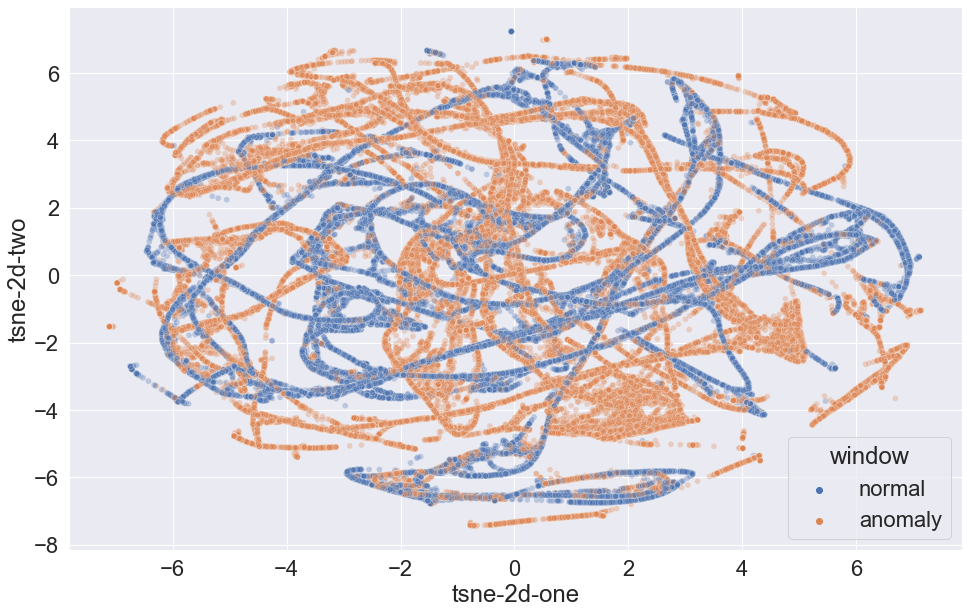
\includegraphics[width=0.33\textwidth]{imgs/chapter_3/std_tsne.png}
    &
   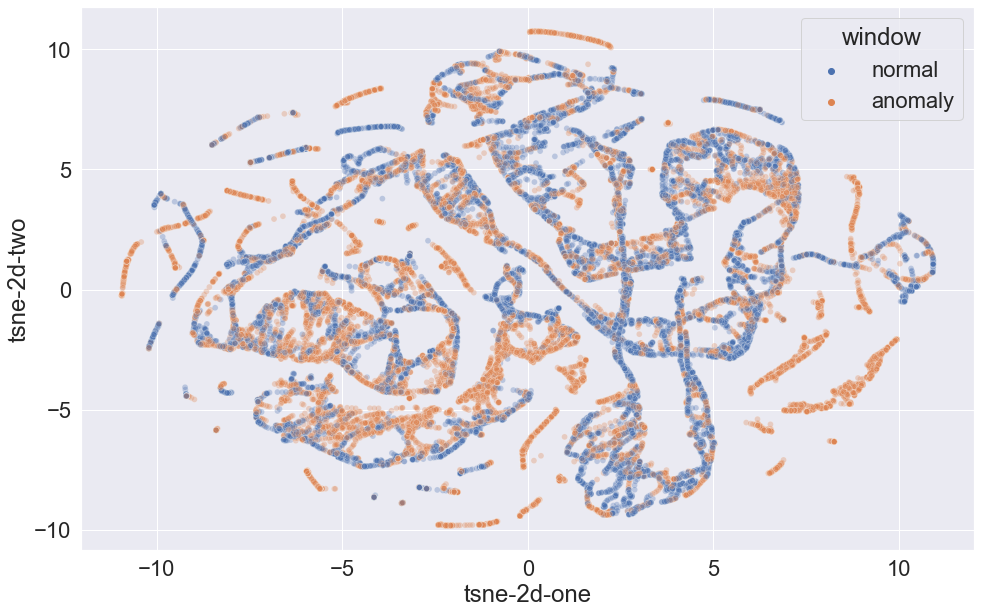
\includegraphics[width=0.33\textwidth]{imgs/chapter_3/gfn_tsne.png}
   &
   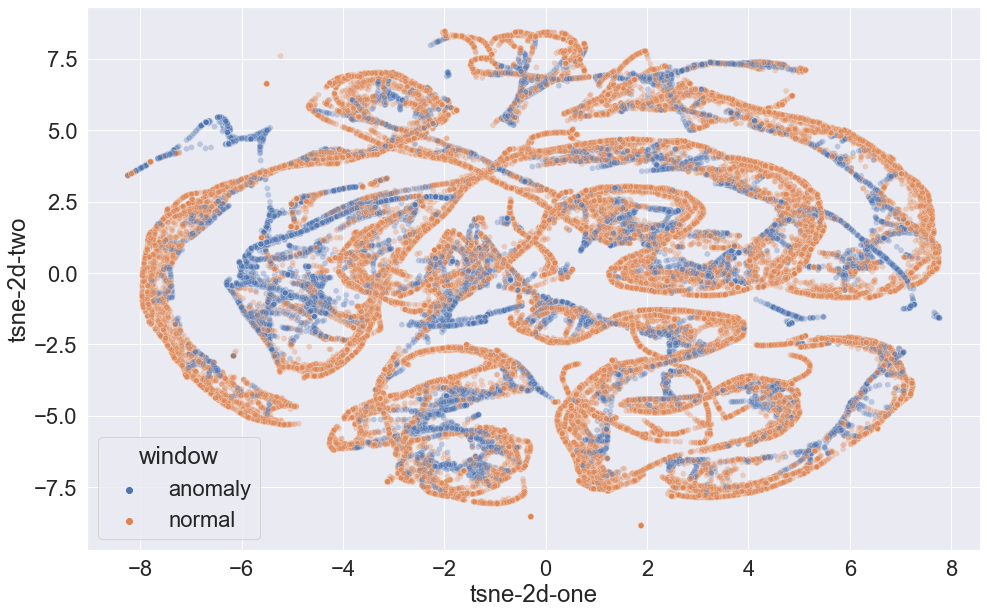
\includegraphics[width=0.33\textwidth]{imgs/chapter_3/xc_tsne.png} \\
     \small \textbf{(a) STD} &
     \small \textbf{(b) GFN} &
     \small \textbf{(c) XC}  \\
  \end{tabular}
  \medskip
  \caption{Visualization of normal and anomalous windows for the three datasets in a two-dimensional space by t-SNE. Normal windows in blue and anomalous windows in orange.}
  \label{fig:chap_3:tsne_viz}
\end{figure*}





% \begin{figure*}[!t]
%   \centering
%   \begin{tabular}{ c @{\hspace{1pt}} c}
%    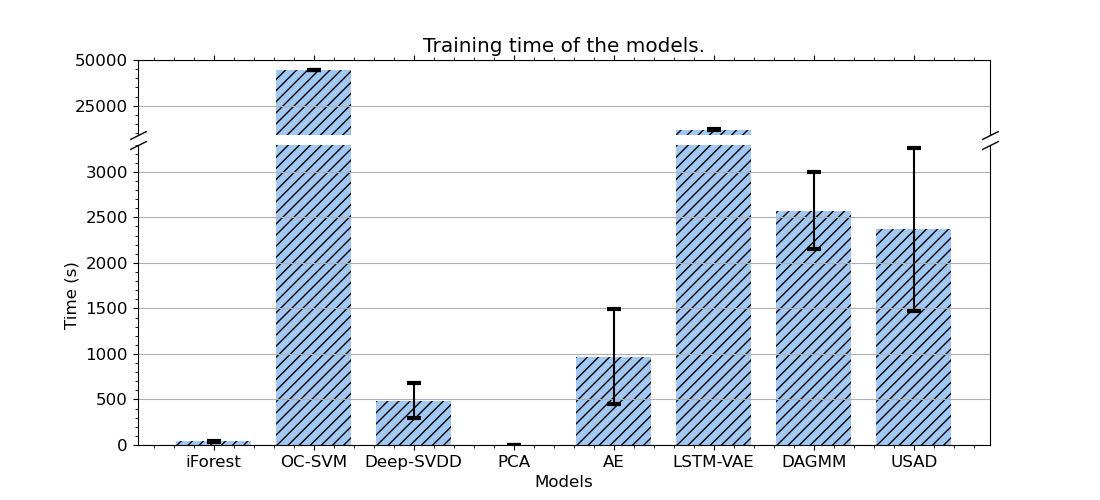
\includegraphics[width=0.5\textwidth]{imgs/chapter_3/train.png}
%     &
    
%    %\medskip
%     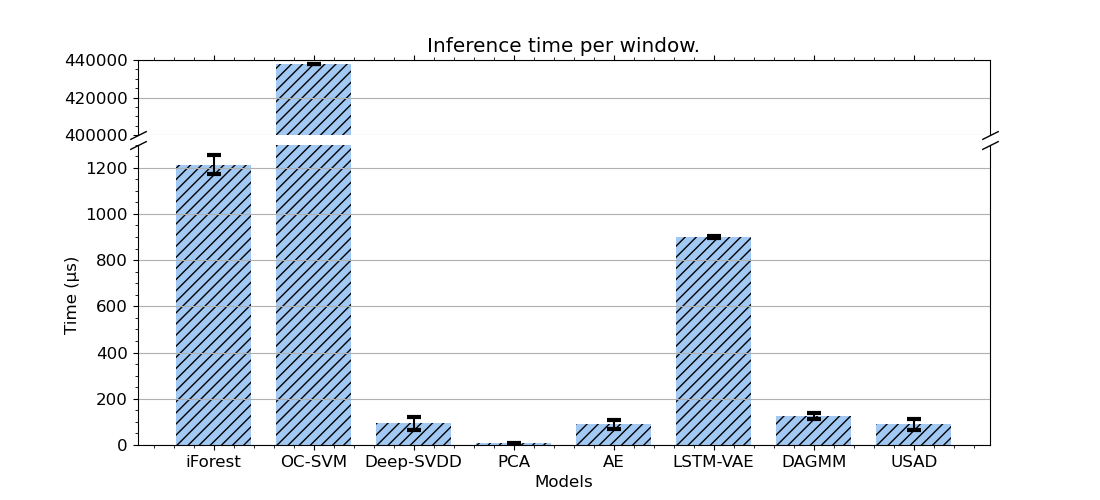
\includegraphics[width=0.5\textwidth]{imgs/chapter_3/inference.png} \\
%      \small \textbf{(a) Training time} &
%     \small \textbf{(b) Inference time per window}  \\
%   \end{tabular}
%   \medskip
%   \caption{Train and inference time.}
%   \label{fig:chap_3:time}
% \end{figure*}




\subsection{Impact of window size}

We also analyze the impact of window size on model performance. The window size represents the duration of the anomalous events that can occur during CG sessions. We choose 3 different values for window size ($p \in \{10,20,30\})$ to have window length representative of user perceptions (50ms, 100ms and 150ms) and to analyze if the models can efficiently detect short or long anomalous events in CG sessions. Fig. \ref{fig:chap_3:mcc_window_size_impact} depicts the MCC score of each model along with the standard deviations with STD dataset. For each model, we represent the impact of the window size $p$ and the contamination ratio $c$ on its performance.


It is worth noting that increasing the window size seems to slightly improve the performance of iForest, DAGMM and USAD models. For instance, the iForest model shows a +30\% increase with $c=0\%$ when the window size varies from 10 to 30. DAGMM and USAD show a moderate increase in performance (i.e., +4\%). Their performance remain better with higher window size regardless of the data contamination ratio. Conversely, OC-SVM, PCA and LSTM-VAE models achieve high performance value with a window size of 10, which decreases as the window size increases. The high variability of Deep-SVDD and the performance variation of AE do not allow to observe a significant pattern.
Our findings remain consistent upon studying the impact of window size on both the GFN and XC datasets: increasing the window size may improve very slightly the performance of iForest and USAD but not the other models.

Apart from the USAD model, to the best of our knowledge, there are no studies on the impact of window size on the AD learning models. Moreover, Audibert et al. \cite{audibert2020usad} showed that increasing the window size has insignificant impact on the performance of USAD, while, in our case, it leads to an increase in model performance. We attribute the performance improvement of iForest and DAGMM (and in the same way the performance degradation of OC-SVM, PCA and AE) to the fact that increasing window sizes leads to the presence of anomalous observations in the training set that may improve (or deteriorate for OC-SVM, PCA and AE) the performance of the models. %Further

\takeaway{The takeaway from these experiments is that detecting longer anomalous events is less efficient for most of the unsupervised models except for iForest, DAGMM and USAD which are able to better learn anomalies over larger windows.}

\begin{figure*}[!t]
    \centering
    %\resizebox{\textwidth}{!}{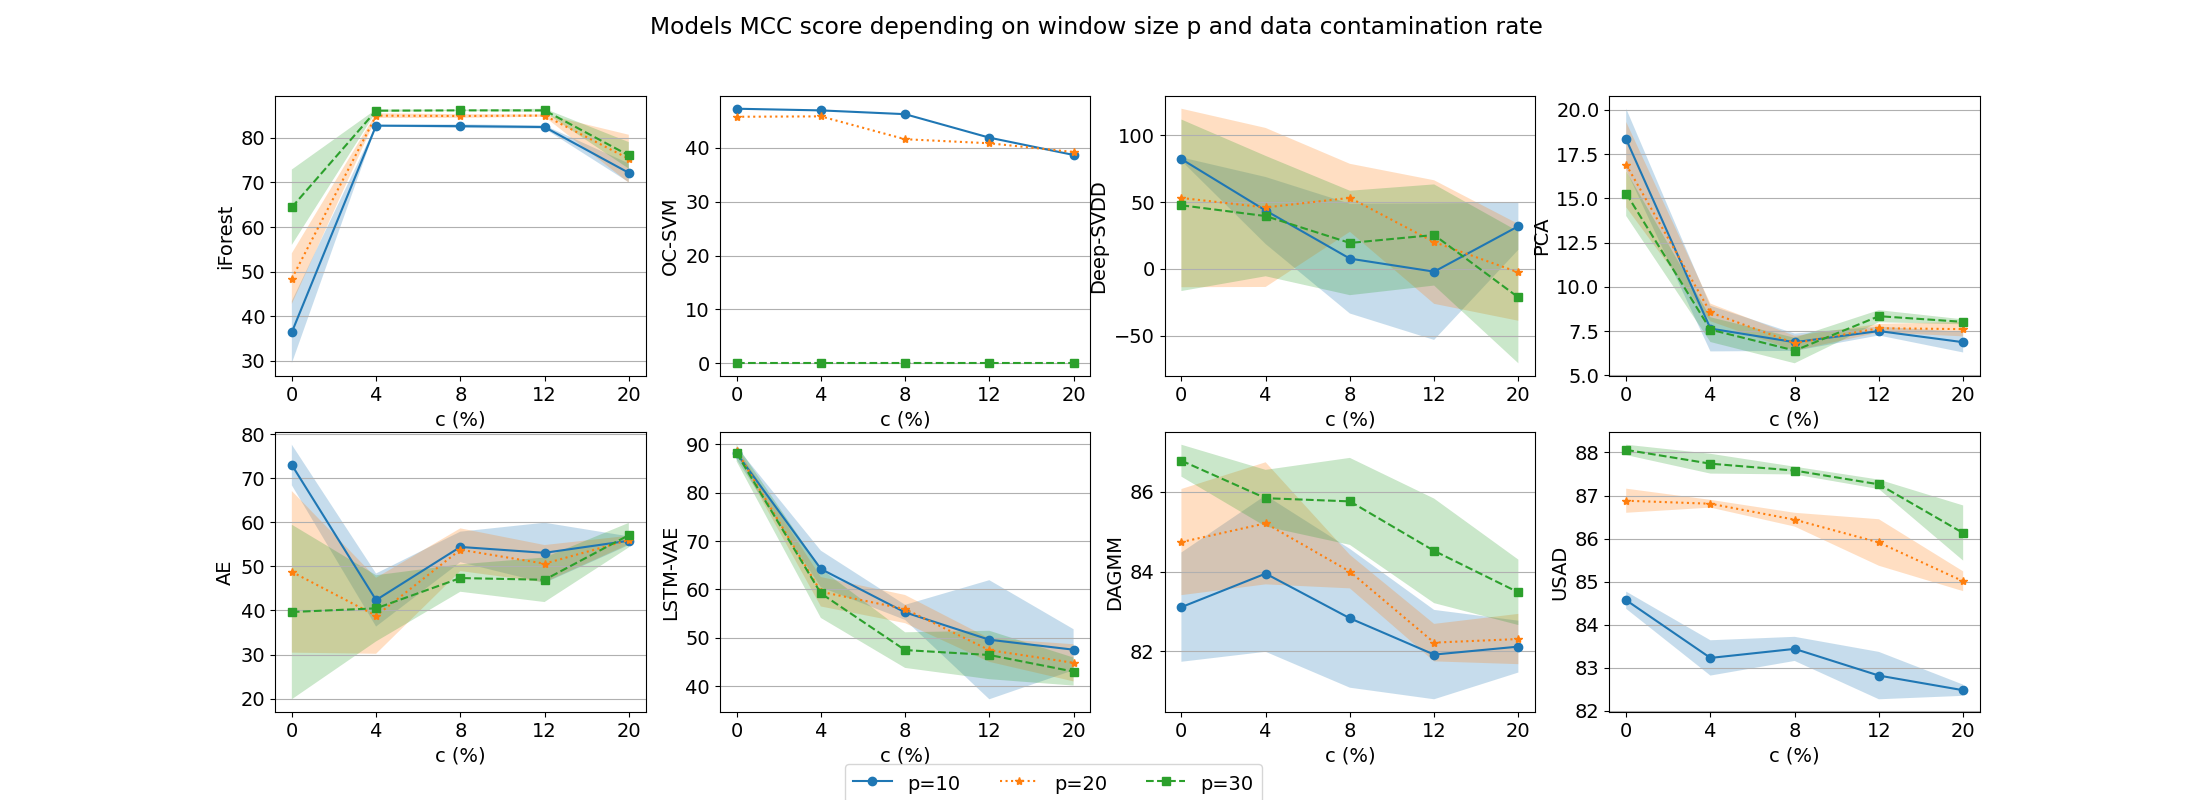
\includegraphics[width=\textwidth]{imgs/chapter_3/window_contamination.png}}
    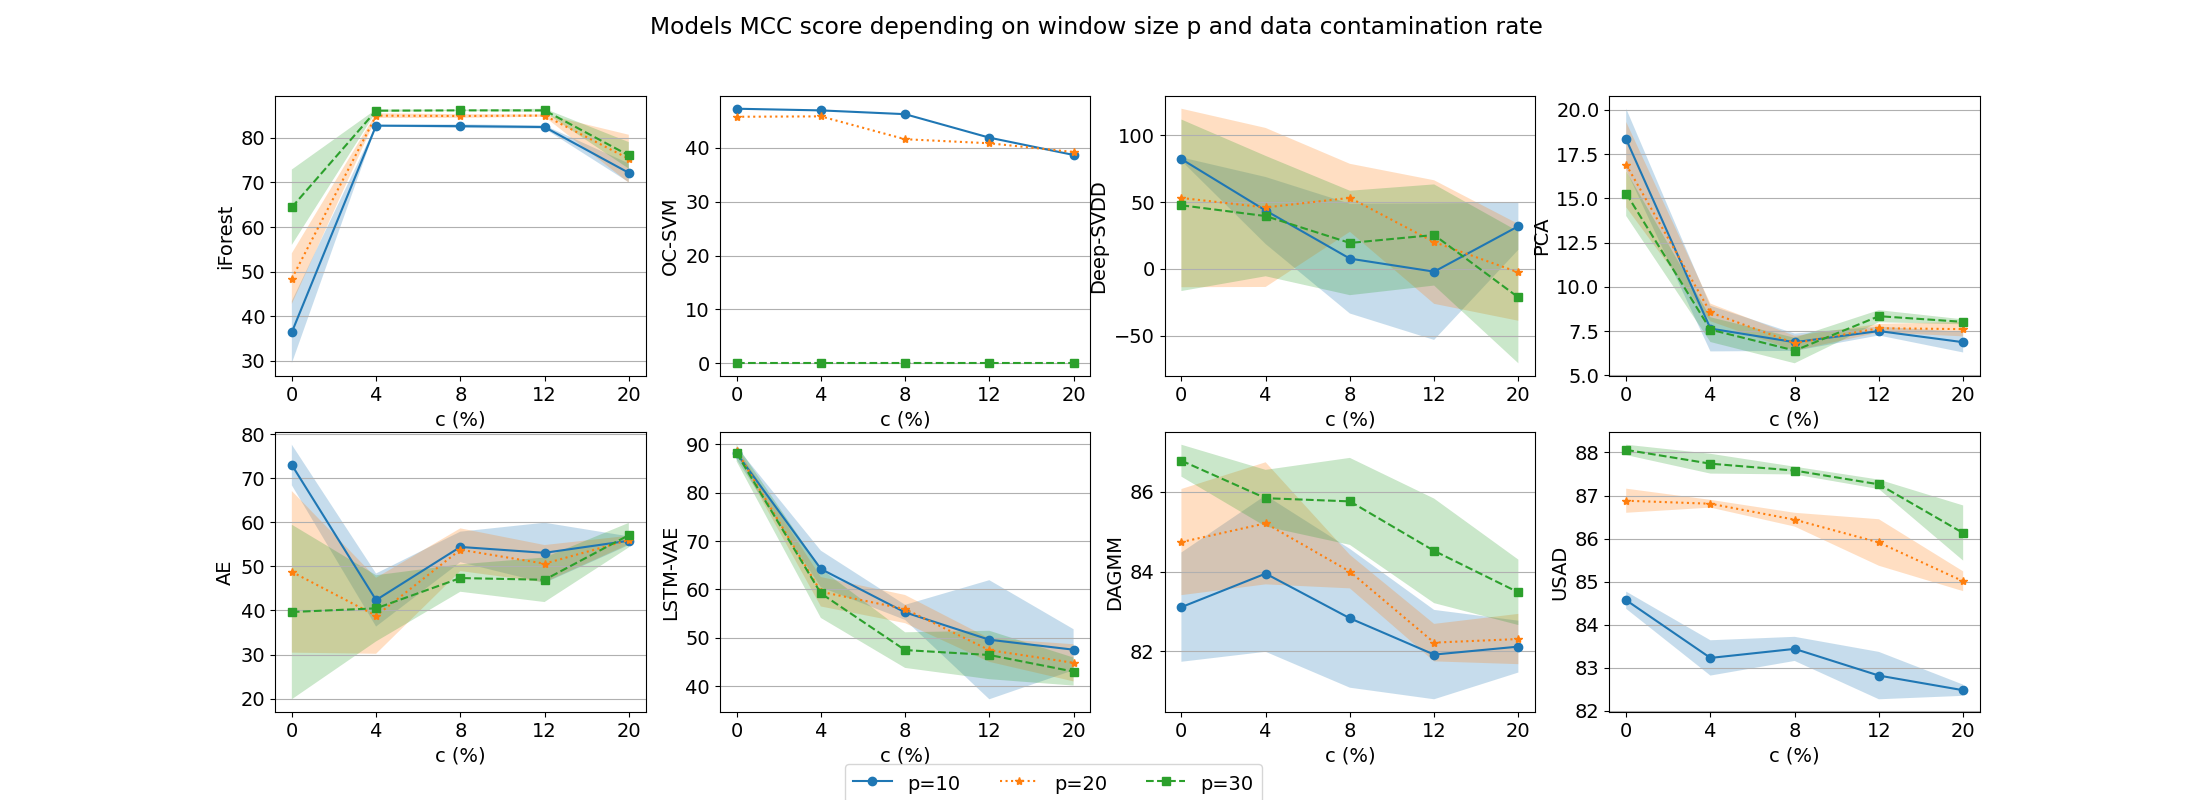
\includegraphics[width=\textwidth]{imgs/chapter_3/window_contamination.png}
    \caption{MCC score of unsupervised ML models with STD dataset according to data contamination ratio $c$ and window size $p$.}
    \label{fig:chap_3:mcc_window_size_impact}
\end{figure*}



\subsection{Computational time performance}

This section analyzes the computational performance of unsupervised ML models. We measure the training time for each model on the training set and compute the average time taken by each model for inference given a window size of 10. The models are trained and tested on a Google Cloud Platform (GCP) VM with 8 CPUs and 30GB RAM. To accelerate the training of LSTM-VAE, a NVIDIA T4 GPU is used.
Fig. \ref{fig:chap_3:time} presents the training and inference times.

PCA takes the lowest training time (i.e., 2s) while iForest training time is 20x longer. Neural networks based models present longer training time ranging from 970s for AE to 2500s for DAGMM. Despite the use of GPU, LSTM-VAE takes 4,6 times longer than DAGMM to complete its training.  The high variability in their training times is due to early stopping strategy that prevents the models from overfitting. The most time consuming model is OC-SVM that takes 44700s for its training. Compared to other shallow models such as iForest, OC-SVM require 1000x longer to train. We make similar observations when comparing the inference time for a window of observations of size $p=10$. Deep learning based models have inference time between 89 and 126µs (except for LSTM-VAE that goes up to 900µs with GPU). Unlike neural network models, shallow models like iForest and OC-SVM take much more inference time, i.e., iForest takes 1213µs and OC-SVM takes 360x longer.

\takeaway{Algorithms with the lowest training/inference time like PCA or with highest training/inference time like OC-SVM or LSTM-VAE do not provide as good qualitative results as iForest, DAGMM and USAD models. The latter present good performance and robustness with reasonable training and test times.}

\begin{figure*}[!t]
  \centering
  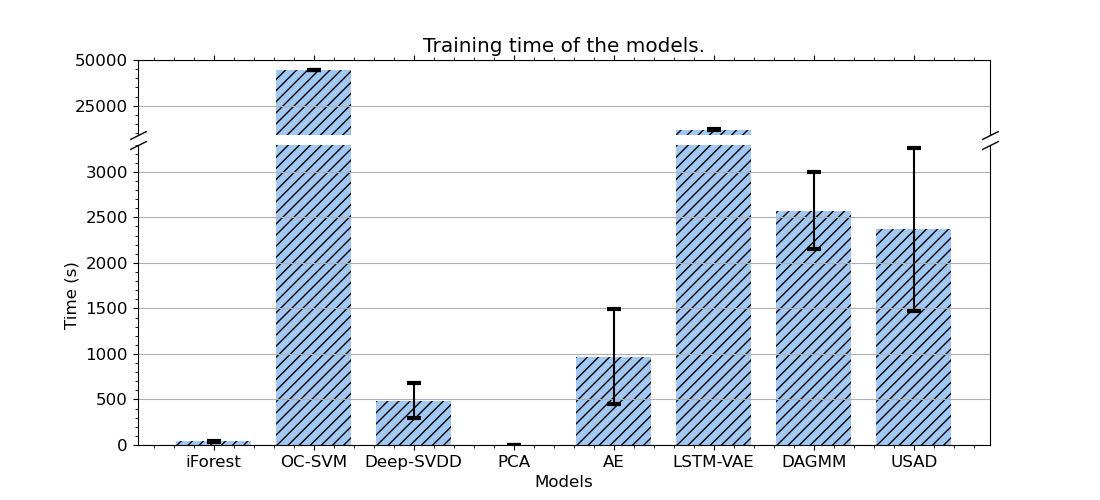
\includegraphics[width=.9\textwidth]{imgs/chapter_3/train.png}
  \small \textbf{(a) Training time} \\
  \medskip
  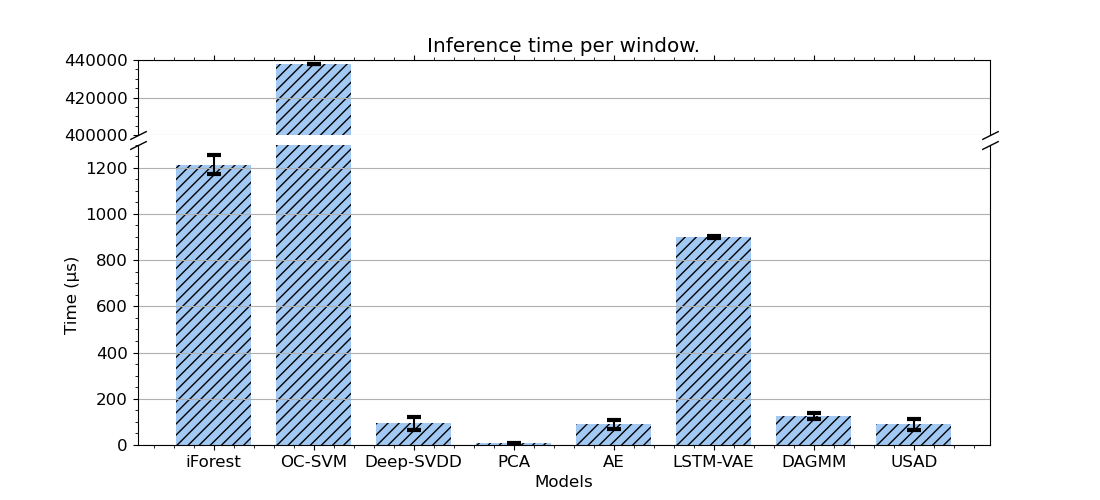
\includegraphics[width=.9\textwidth]{imgs/chapter_3/inference.png}
  \small \textbf{(b) Inference time per window} \\
  \medskip
  \caption{Train and inference time.}
  \label{fig:chap_3:time}
\end{figure*}


